\documentclass[letterpaper]{article} % DO NOT CHANGE THIS
\usepackage{aaai2027}  % DO NOT CHANGE THIS
\usepackage[hyphens]{url}  % DO NOT CHANGE THIS
\usepackage{graphicx} % DO NOT CHANGE THIS
\urlstyle{rm} % DO NOT CHANGE THIS
\def\UrlFont{\rm}  % DO NOT CHANGE THIS
\usepackage{natbib}  % DO NOT CHANGE THIS AND DO NOT ADD ANY OPTIONS TO IT
\usepackage{caption} % DO NOT CHANGE THIS AND DO NOT ADD ANY OPTIONS TO IT
\frenchspacing  % DO NOT CHANGE THIS
\usepackage{booktabs}
\usepackage{amsmath}
\setcounter{secnumdepth}{2}
\pdfinfo{
/TemplateVersion (2027.1)
}

\title{Lesion or Location? Negative Controls for Lesion-Level\\Fidelity Evaluation in Accelerated Knee MRI}

\author{
    Sachin Mote\textsuperscript{\rm 1},
    Pranjali Changadeo Pingale\textsuperscript{\rm 2},
    Alicem Koyun\textsuperscript{\rm 2}
}
\affiliations{
    \textsuperscript{\rm 1}George Mason University, Fairfax, VA, United States\\
    \textsuperscript{\rm 2}Westcliff University, Irvine, CA, United States\\
    sachinmoteofficial@gmail.com, pranjalipingale@gmail.com, alicemkoyun@gmail.com
}

\begin{document}
\maketitle

\begin{abstract}
Accelerated MRI reconstructions are increasingly scored inside
radiologist-annotated lesion boxes, on the premise that a box isolates what
happens to the finding. We test that premise with linear reconstructions,
which have no learned prior that could remove or invent pathology and so
provide a setting in which strong lesion-specific loss is not expected. On
fastMRI knee data with fastMRI+ annotations (217 boxes, 18 patients),
reconstructed with unregularised CG-SENSE and zero-filling at nominal 2-, 4-
and 8-fold acceleration (effective about 1.7, 2.7 and 3.8), we find three
problems. First, box registration fails silently: with the wrong vertical
origin, none of 146 meniscus and cartilage boxes lies near the joint line, yet
the analysis yields significant, plausible lesion effects. Second, the
comparator drives the estimate. Under CG-SENSE at nominal 4-fold acceleration,
the mean patient-level lesion effect is $+0.046$ SSIM against size-matched
tissue, $+0.058$ against appearance-matched tissue and $-0.054$ against the
same box on other slices of the same patient; the size-matched estimate
exceeds the same-position estimate in every one of 18 patients (mean
difference 0.100). Third, a
per-finding deficit that passes a patient-level test (cartilage defects,
$-0.179$, 8 of 9 patients) is not supported against nearby slices, and within
the same boxes it grows with comparator distance. Against the adjacent slice
the pooled effect is $0.000$ $[-0.013, +0.012]$, but those 36 boxes are
mostly edge slices of multi-slice lesions. The contribution is an evaluation
protocol: verify registration, report effects against several comparators
including one that holds anatomy fixed, compare them with a lesion-free noise
floor, and make the patient the unit of inference.
\end{abstract}

\begin{links}
\link{Code}{https://github.com/sachinmoteofficial/AAAI27}
\end{links}

\section{Introduction}

Accelerated MRI acquires a fraction of $k$-space and reconstructs the rest,
which shortens examinations and widens access to scanner time. Whether the
shortened examination is still diagnostic depends on whether the
reconstruction preserves findings, yet reconstructions are compared mainly by
SSIM or PSNR over the whole image \citep{zbontar2018fastmri,muckley2021results}.
Whole-image scores track radiologists' quality ratings only loosely
\citep{mason2020iqm}, and the fastMRI challenges documented meniscal tears and
small osteophytes lost by reconstructions that scored well
\citep{knoll2020challenge}.

Radiologist bounding boxes for fastMRI, released as fastMRI+
\citep{zhao2022fastmriplus}, make a finer evaluation possible: compute the
metric inside each lesion box and compare it with tissue elsewhere. This
lesion-box evaluation needs no reader study and no trained detector, which
makes it attractive for comparing many reconstructions. It also matters for
reconstruction without raw data: methods such as CUPID
\citep{alcalar2025cupid} train on images exported by the scanner and use an
unregularised parallel-imaging reconstruction as network input and inside the
consistency operator, so how that reconstruction treats lesions bears on what
such networks see.

A lesion-box comparison is only as good as its comparator. A lesion box
differs from a tissue box elsewhere in at least three ways: it contains a
finding, it sits at a particular anatomical position, and it covers tissue of
a particular brightness and texture. SSIM depends on local mean and variance
\citep{wang2004ssim}, and parallel-imaging error varies across the image, so
position and appearance can produce a lesion effect on their own. We
separate these factors with negative controls, using linear reconstructions
as a test bed: zero-filling and unregularised CG-SENSE have no learned prior
that could remove or invent a finding, so a large lesion-specific effect
would be surprising, and a comparator that reports one is suspect.

Our contributions are:
\begin{itemize}
\item A registration check for fastMRI+ boxes, and evidence from our own
earlier analysis that a coordinate-origin error yields significant,
plausible and meaningless lesion effects.
\item A comparison of comparators on the same 217 boxes: size-matched and
appearance-matched tissue on the same slice, and the same box on other slices
of the same patient, stratified by slice distance.
\item Evidence that the estimated lesion effect changes sign with the
comparator, that a significant per-finding effect depends on comparator
distance within the same boxes, and that the closest comparator available,
the adjacent slice, covers mainly lesion edges.
\item An evaluation protocol for lesion-box metrics: registration check,
several comparators, a lesion-free noise floor and patient-level inference.
\item Code, subject splits and per-region results.
\end{itemize}

\begin{figure*}[t]
\centering
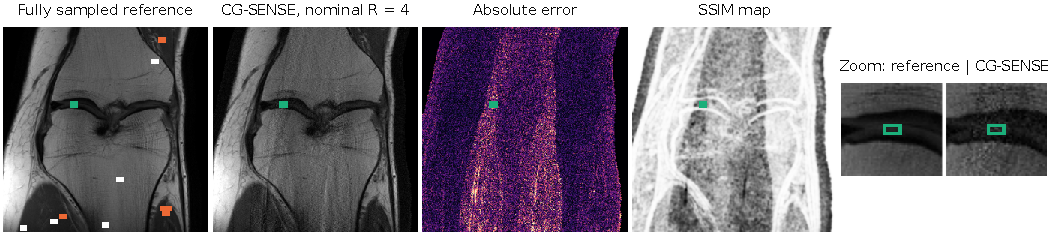
\includegraphics[width=\textwidth]{figures/fig_example.pdf}
\caption{\textbf{Example and comparators} (patient file1000831, slice 21,
partial-thickness cartilage defect). Left to right: fully sampled reference,
CG-SENSE at nominal $R=4$, absolute error, SSIM map, and a zoom of the box.
Teal: lesion box (in-box SSIM 0.47). White: size-matched controls (mean
0.50). Orange: appearance-matched controls. The same coordinates on slice 14,
seven slices away, score 0.96; this distance effect is the subject of
Section~\ref{sec:dist}.}
\label{fig:example}
\end{figure*}

\section{Related Work}

\textbf{Clinical evaluation of accelerated reconstruction.} Reader studies
remain the reference standard; deep-learning reconstruction of knee MRI was
interchangeable with conventional images for detecting internal derangement
\citep{recht2020interchangeability}. Reader studies are expensive and rarely
used to compare methods, so image metrics dominate, although SSIM correlated
no better than RMSE with radiologists' scores \citep{mason2020iqm}.

\textbf{Pathology-aware quantitative evaluation.} \citet{zhao2021pipeline}
coupled reconstruction with a meniscal-tear detector and found detection
failed on low-SNR CG-SENSE and on heavily accelerated reconstructions.
\citet{chen2023pathology} compared metrics inside fastMRI+ brain boxes with
normal patches for an end-to-end variational network and reported larger
losses in pathological regions. \citet{morshuis2025mind} trained a detector on
fastMRI+ knee data to show that reconstructions can miss small, rare
pathologies, and \citet{cheng2020fnaf} showed that small synthetic features
are systematically lost by trained networks. These studies compare lesion
regions with normal regions or count detections; we ask whether such
lesion-versus-normal differences reflect the finding or the comparator.

\textbf{Reconstruction without fully sampled data.} Self-supervised methods
such as SSDU \citep{yaman2020ssdu} remove the need for fully sampled
references, and CUPID \citep{alcalar2025cupid} removes the need for raw
$k$-space. Both rely on parallel imaging
\citep{pruessmann1999sense,griswold2002grappa}, which motivates our choice of
CG-SENSE.

\section{Data and Reconstruction}

\subsection{Cohort}
We use the fastMRI multi-coil knee validation set
\citep{zbontar2018fastmri,knoll2020fastmri}, restricted to coronal
proton-density scans without fat suppression and to the 49 volumes with 368
phase-encode lines, so that every scan has the same matrix. Volumes were split
by subject into 15 for a future training experiment, 19 for testing and 15
unused. Of the 19 test subjects, 18 carry at least one fastMRI+ bounding box;
the remaining subject has only a study-level label. We score the central 20
slices of each test volume (380 slices); 140 of them carry 217 boxes in nine
finding categories. One patient contributes 35 boxes.

\subsection{Registering the annotations}
fastMRI+ boxes are given as $(x, y, w, h)$ on the $320\times320$
root-sum-of-squares image. We crop reconstructions to the same field and
convert with a bottom-left origin, $\text{row}_\text{top} = 320 - y - h$.
Because an origin error causes no crash and no visibly odd numbers
(Section~\ref{sec:reg}), we verify registration automatically. Meniscus-tear
and cartilage-defect boxes must lie on the joint line, so for each such box
we locate the joint line as the darkest row of the smoothed intensity profile
over the box's columns and record its distance from the box centre. The
pipeline stops if fewer than 80\% of these boxes lie within 15 pixels.

\begin{figure}[t]
\centering
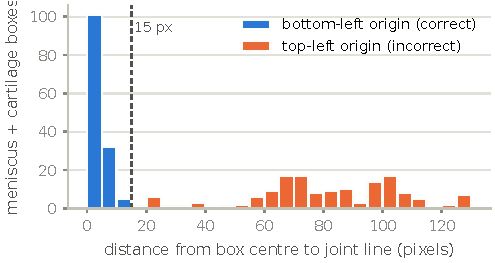
\includegraphics[width=\columnwidth]{figures/fig_registration.pdf}
\caption{\textbf{Registration check.} Distance from each meniscus-tear or
cartilage-defect box centre ($n=146$) to the joint line under the correct
(bottom-left) and an incorrect (top-left) vertical origin.}
\label{fig:reg}
\end{figure}

\subsection{Undersampling and reconstruction}
Readout oversampling is removed in the image domain ($640\to320$). Coil
sensitivities are estimated from a Hann-windowed block of 24 autocalibration
lines, normalised by root-sum-of-squares and zeroed below 2\% of the maximum;
the combined reference agrees with the fastMRI reconstruction (correlation
0.999, NRMSE 0.062). We keep every $R$th phase-encode line plus the
autocalibration block and, as in the CUPID code, mark zero-padded lines as
known. The realised sampled fractions at nominal $R=2,4,8$ are 0.58, 0.37 and
0.27, so nominal $R=2,4,8$ correspond to effective accelerations of about
1.7, 2.7 and 3.8. We
reconstruct with the zero-filled adjoint and with unregularised CG-SENSE (30
iterations, zero initialisation), the configuration the CUPID code uses for
its parallel-imaging image. Whole-image SSIM under CG-SENSE is 0.959, 0.721
and 0.470 at nominal $R=2,4,8$ (zero-filled 0.770 at $R=4$). Unless stated, results
are for nominal $R=4$.

\section{Comparators and Statistics}

For each box we compute an SSIM map \citep{wang2004ssim} against the fully
sampled reference (Gaussian window, $\sigma=1.5$, dynamic range set by the
slice maximum) and average it inside the box; PSNR uses the in-box squared
error with the same peak. Each lesion box is compared with three comparators
(Figure~\ref{fig:example}).

\textbf{Size-matched (SM).} Five boxes of identical size drawn at random on
the same slice inside an eroded tissue mask ($>8\%$ of the slice maximum),
disjoint from all annotations. This is the comparison lesion-box studies
usually make.

\textbf{Appearance-matched (AM).} Among up to 2{,}000 same-size candidates
inside the body on the same slice, the five closest to the lesion box in
standardised mean intensity, Michelson contrast and standard deviation.

\textbf{Same position (SP).} The identical box at identical coordinates on
each slice of the same patient, within the scored band, that carries no
fastMRI+ annotation (2{,}147 placements; 215 boxes have at least one). SP
holds position exactly but anatomy only approximately, and less so the
further the comparator slice lies from the lesion slice. We therefore report
SP for all slices and stratified by slice distance $d$: adjacent ($d=1$) and
nearby ($d\le3$).

The \emph{lesion effect} is in-box SSIM of the lesion box minus the mean over
its comparator boxes; negative values mean the lesion is reconstructed less
faithfully. Boxes are clustered within patients, and one patient contributes
35 boxes, so the patient is the unit of inference throughout. We average
effects within each patient and report the mean of the patient means, a
95\% percentile bootstrap interval over patients (5{,}000 resamples), the
number of patients with positive and negative means, and a Wilcoxon
signed-rank test on the patient means. We give no intervals for categories
with fewer than three patients and no tests for fewer than five.

Two further analyses use the same estimator. To test whether comparators
disagree, we take the difference between a box's effect under two comparators
and average it within patients. To separate comparator distance from box
composition, we compare, for the same box, its effect against near and against
far same-position slices. Finally, a \emph{lesion-free noise floor} measures how
much in-box SSIM changes between adjacent slices from anatomy alone: for every
SP box we take pairs of adjacent unannotated slices at the same coordinates
and record the absolute difference in SSIM.



\section{Results}

\begin{figure}[t]
\centering
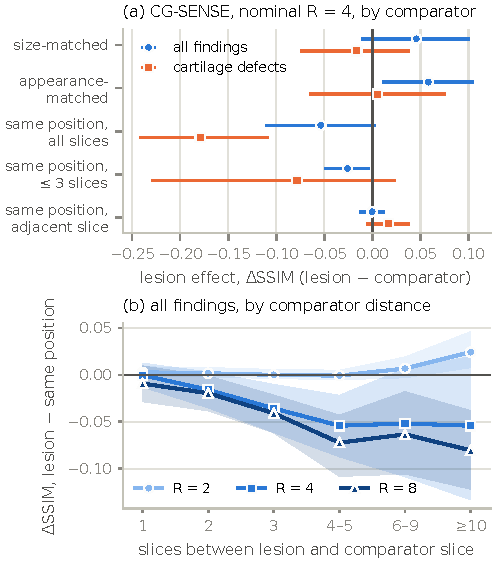
\includegraphics[width=\columnwidth]{figures/fig_comparators.pdf}
\caption{\textbf{The lesion effect depends on the comparator.} (a) CG-SENSE at
nominal $R=4$: lesion effect for all findings (18 patients) and for
partial-thickness cartilage defects (9 patients) against each comparator.
(b) Same-position lesion effect for all findings by distance to the
comparator slice, at nominal $R=2,4,8$. Points are means of patient means;
bars and bands are 95\% bootstrap intervals over patients. Each distance bin
contains a different mix of boxes (Section~\ref{sec:dist}).}
\label{fig:comp}
\end{figure}

\subsection{Registration errors are silent}
\label{sec:reg}

With the bottom-left origin, 93.8\% of meniscus-tear boxes (median distance
2.0 pixels, $n=97$) and 95.9\% of cartilage-defect boxes (median 5.0 pixels,
$n=49$) lie within 15 pixels of the joint line. With a top-left origin the same
boxes fall in femoral or tibial marrow and none lies within 15 pixels (median
80.0 and 85.5 pixels; Figure~\ref{fig:reg}).

The misregistered boxes nonetheless produce results that look like findings.
Against size-matched controls, CG-SENSE scores them higher than tissue
($+0.038$ SSIM, region-level Wilcoxon $p=4.6\times10^{-5}$), zero-filling
scores them lower ($-0.024$, $p=1.9\times10^{-7}$), and SSIM and PSNR disagree
in sign. An earlier version of this study made this error and interpreted
these numbers as properties of pathology. Nothing in them indicates that the
boxes contain marrow; only an anatomical check does. Region-level tests
compound the problem: treating 217 boxes from 18 patients as independent, the
CG-SENSE effect looked overwhelming, whereas at the patient level it was
$p=0.099$.



\subsection{The comparator sets the sign}




With correct registration, the lesion effect depends on which comparator is
used (Table~\ref{tab:main}, Figure~\ref{fig:comp}a). Under CG-SENSE, lesion
boxes score higher than size-matched tissue on the same slice ($+0.046$).
Lesion boxes sit on the meniscus, cartilage and ligaments and are much darker
and higher in contrast than size-matched controls (mean intensity 0.127 vs.\
0.335, Michelson contrast 0.88 vs.\ 0.50). Appearance matching closes most of
that gap (0.148, 0.85) but not the effect ($+0.058$), because lesions and
their appearance-matched controls still lie in different places. Holding
position fixed reverses the sign: the same box on unannotated slices of the
same patient scores higher than the lesion ($-0.054$, 12 of 18 patients
negative). None of these three estimates is individually conclusive at the
patient level, but the disagreement between them is: for the same boxes, the
size-matched estimate exceeds the all-slice same-position estimate by
$+0.100$ $[+0.072, +0.131]$, in all 18 patients ($p<0.001$), and the
appearance-matched estimate exceeds it by $+0.112$ (17 of 18). Under
zero-filling the comparators agree ($-0.005$ $[-0.032, +0.022]$), so how much
the comparator matters depends on the reconstruction as well.

\begin{table}[t]
\centering
\footnotesize
\setlength{\tabcolsep}{2.5pt}
\begin{tabular}{lrcc}
\toprule
Comparator & $\Delta$SSIM & 95\% CI & pts $+$/$-$ ($p$) \\
\midrule
\multicolumn{4}{l}{\emph{CG-SENSE}} \\
Size-matched & $+0.046$ & $[-0.011, +0.101]$ & 12/6 (0.13) \\
Appearance-matched & $+0.058$ & $[+0.011, +0.105]$ & 11/7 (0.05) \\
Same position, all & $-0.054$ & $[-0.111, +0.003]$ & 6/12 (0.12) \\
Same position, $d\le3$ & $-0.026$ & $[-0.050, -0.003]$ & 6/12 (0.14) \\
Same position, $d=1$ & $0.000$ & $[-0.013, +0.012]$ & 8/10 (0.90) \\
\midrule
\multicolumn{4}{l}{\emph{Zero-filled}} \\
Size-matched & $+0.029$ & $[+0.003, +0.055]$ & 12/6 (0.04) \\
Appearance-matched & $+0.022$ & $[-0.004, +0.049]$ & 12/6 (0.13) \\
Same position, all & $+0.034$ & $[+0.009, +0.057]$ & 12/6 (0.03) \\
Same position, $d\le3$ & $+0.015$ & $[-0.001, +0.033]$ & 9/9 (0.32) \\
Same position, $d=1$ & $+0.005$ & $[-0.008, +0.018]$ & 10/8 (0.32) \\
\bottomrule
\end{tabular}
\caption{\textbf{Lesion effect by comparator} at nominal $R=4$ (217 boxes, 18
patients; same-position rows use the 215, 103 and 36 boxes with a comparator
slice at that distance). $\Delta$ is lesion minus comparator in-box SSIM, as
the mean of patient means, with a 95\% bootstrap interval over patients; $p$
is a Wilcoxon test on the 18 patient means. The interval and the test can
disagree near the boundary (rows 2 and 4), because one summarises the mean
and the other the signed ranks.}
\label{tab:main}
\end{table}

\subsection{Comparator distance}
\label{sec:dist}

Binned by the distance between the lesion slice and the comparator slice, the
same-position effect becomes more negative with distance
(Figure~\ref{fig:comp}b): under CG-SENSE at nominal $R=4$ it is $0.000$ at
one slice, $-0.036$ at three and about $-0.05$ beyond three. In
Figure~\ref{fig:example}, the comparator seven slices away scores 0.96
against the lesion's 0.47. Two things change with distance, however. Distant
slices cut through different anatomy at the same coordinates, and the bins
contain different boxes: a box whose nearest unannotated slice is far away
usually lies in the middle of a lesion that spans several slices. Comparing
near and far comparators for the same box separates the two. Pooled over
findings, far ($d\ge4$) comparators give a more negative effect than the
adjacent slice for the same box ($-0.037$ $[-0.110, +0.037]$, 34 boxes, 17
patients, $p=0.43$): the direction agrees with Figure~\ref{fig:comp}b but the
contrast is not conclusive.

The adjacent-slice comparison is the closest available, and against it the
lesion effect is $0.000$ $[-0.013, +0.012]$ under CG-SENSE and $+0.005$
$[-0.008, +0.018]$ under zero-filling, with patients split evenly; PSNR
agrees ($-0.14$\,dB $[-0.53, +0.22]$). Two caveats limit what this shows.
First, 34 of the 36 boxes have an annotation on the neighbouring slice, so
they are edge slices of multi-slice lesions, and they are smaller than average
(median 336 vs.\ 495 pixels). Second, adjacent slices differ even without a
lesion: at the same coordinates on pairs of adjacent unannotated slices
(1{,}812 pairs), in-box SSIM differs by a median of 0.029 (95th percentile
0.150). The lesion-versus-adjacent differences lie within this noise floor
(median 0.021, 95th percentile 0.084). Under zero-filling the noise floor is
similar (median 0.028, 95th percentile 0.118), and the lesion-versus-adjacent
differences again lie within it (median 0.032).

\subsection{A per-finding result that is not supported}

Per finding, the same-position design produces a result that would pass
review. Against same-position boxes on all slices, partial-thickness
cartilage defects score $-0.179$ $[-0.242, -0.108]$ SSIM under CG-SENSE,
worse in 8 of 9 patients (Wilcoxon $p=0.008$); PSNR agrees ($-4.1$\,dB, 8 of
9). Against size-matched or appearance-matched tissue, the same boxes show
nothing ($-0.016$ and $+0.005$). Against nearby slices the deficit is no
longer supported: $-0.078$ $[-0.229, +0.024]$ for $d\le3$ (7 patients) and
$+0.017$ $[-0.006, +0.039]$ for $d=1$ (4 patients). Unlike the pooled set,
cartilage defects show the distance dependence within the same boxes: far
($d\ge6$) comparators give an effect $0.157$ lower than near ($d\le3$) ones
$[-0.270, -0.044]$, in 6 of 7 patients (22 boxes, $p=0.047$). The all-slice
deficit therefore reflects the comparator at least as much as the finding.
Meniscus tears, the largest category, show no deficit nearby ($-0.018$
$[-0.054, +0.010]$ for $d\le3$, 14 patients). We had singled out cartilage
defects after an exploratory look at the same data, so the all-slice result
should in any case have been treated as a hypothesis.

\begin{table}[t]
\centering
\footnotesize
\setlength{\tabcolsep}{2.4pt}
\begin{tabular}{lrrrrr}
\toprule
& & & \multicolumn{3}{c}{Same position} \\
\cmidrule(lr){4-6}
Finding (boxes, pts) & SM & AM & all & $d\le3$ & $d=1$ \\
\midrule
Cartilage (49, 9) & $-0.016$ & $+0.005$ & $\mathbf{-0.179}$ & $-0.078$ & $+0.017$ \\
Meniscus (97, 15) & $+0.046$ & $+0.048$ & $-0.068$ & $-0.018$ & $-0.004$ \\
MCL (11, 5) & $\mathbf{+0.163}$ & $\mathbf{+0.132}$ & $+0.020$ & $\mathbf{-0.025}$ & $-0.007$ \\
\bottomrule
\end{tabular}
\caption{\textbf{Lesion effect by finding} (CG-SENSE, nominal $R=4$,
$\Delta$SSIM, mean of patient means): partial-thickness cartilage defect,
meniscus tear and low--moderate MCL sprain. Bold: 95\% bootstrap interval
over patients excludes zero. The same-position subsets contain fewer patients
($d\le3$ and $d=1$: cartilage 7 and 4, meniscus 14 and 12, MCL 4 and 4), so
the MCL $d\le3$ interval rests on four patients. Categories with fewer than
five patients (effusion, ACL and LCL sprains, retinaculum, displaced meniscal
tissue; 60 boxes) are not shown.}
\label{tab:labels}
\end{table}

\subsection{Acceleration}

At nominal $R=2$ all lesion effects are small (size-matched $+0.014$, same
position $+0.013$). At nominal $R=8$ the size-matched effect turns negative
($-0.026$ $[-0.056, +0.005]$), and the same-position effect is negative for
all slices ($-0.068$ $[-0.098, -0.038]$, 16 of 18 patients, $p=0.0004$) and
for $d\le3$ ($-0.031$ $[-0.050, -0.012]$, 14 of 18, $p=0.007$), but not for
the adjacent slice ($-0.009$ $[-0.028, +0.010]$). At $R=8$, where whole-image
SSIM falls to 0.47, some lesion-specific loss is plausible, but this design
cannot separate it from through-plane anatomy and lesion extent.

\section{Discussion}

Lesion-box metrics are a reasonable step toward clinically relevant
evaluation, but the unit of interest is the finding, not the box. Two things
stand between them. The first is registration, whose failure is silent: our
misregistered analysis produced significant effects, a sign reversal between
reconstructions and a disagreement between metrics, all of which read
naturally as findings. The second is the comparator. Lesions sit on anatomy
that is darker, higher in contrast and differently placed than tissue drawn
elsewhere on the slice, and SSIM responds to all three. Under CG-SENSE the
estimated lesion effect ranged from $+0.058$ to $-0.054$ depending only on the
comparator, the comparators disagreed in every patient, and a per-finding
deficit significant at the patient level depended on comparator distance
within the same boxes.

Linear reconstructions make these problems visible because they have no
learned prior that could remove or invent a finding. They are not immune to
content: thin, high-contrast structures lose more detail than smooth tissue,
and appearance matching only partly accounts for that. But a large
lesion-specific effect from zero-filling or unregularised CG-SENSE should be
treated first as a property of the comparator. Our contribution is therefore
the evaluation protocol, not the near-null result: the protocol should be
applied, unchanged, to learned reconstructions, where lesion-specific loss is
the real concern.

No comparator we tried isolates the finding completely. Same-slice
comparators differ in position and appearance; same-position comparators
differ in anatomy, increasingly with distance, and the nearest ones cover
mainly lesion edges, which are smaller and possibly less conspicuous than
lesion centres. Against the adjacent slice we see no lesion-specific loss at
nominal $R\le4$, but that conclusion applies to lesion edges, and the
differences lie within a lesion-free noise floor of about 0.03 SSIM.

For evaluating reconstructions, including those trained without raw data, we
suggest four inexpensive practices: verify box registration against anatomy
before computing any metric; report effects against several comparators,
including one that holds position and anatomy fixed, and state which part of
each lesion the comparison covers; compare effects with a lesion-free noise
floor; and make the patient, not the box, the unit of inference.

\textbf{Limitations.} Eighteen patients, of whom only three finding
categories contribute five or more, limit per-finding conclusions, and the
nearest-slice comparisons have few boxes. Adjacent slices still differ
through-plane, and fastMRI+ is not exhaustive, so an unannotated slice is not
necessarily normal. Many boxes are small (median 325 pixels for cartilage
defects), so in-box SSIM is influenced by pixels within a few window widths of
the box edge. Coil maps are estimated from the autocalibration block rather
than with ESPIRiT \citep{uecker2014espirit}. We evaluate two linear
reconstructions; learned reconstructions \citep{hammernik2018variational} may
behave differently, and the training split we release is intended for that
comparison.

\section{Conclusion}

Comparing lesion boxes with tissue elsewhere measures where lesions are and
what they look like as much as whether reconstruction preserves them, and an
undetected registration error can make such comparisons look meaningful. On
linear reconstructions of fastMRI knee data at nominal 4-fold acceleration
(effective about 2.7), comparator choice shifted the estimated lesion effect
by 0.10 SSIM on average, in the same direction in every patient, and against the closest comparator, which
covers mainly lesion edges, we found no lesion-specific fidelity loss beyond
a lesion-free noise floor. Lesion-box evaluations of learned reconstructions
should report a registration check, several comparators, a noise floor and
patient-level inference.

\section*{Data and Ethics Statement}
This is a secondary analysis of de-identified, publicly released data. fastMRI
data were obtained from NYU Langone Health under the fastMRI data use
agreement \citep{zbontar2018fastmri,knoll2020fastmri}, and fastMRI+
annotations from their public release \citep{zhao2022fastmriplus}. No imaging
data are redistributed; the repository contains code, subject splits and
derived per-region results.

\section*{Acknowledgments}
Data used in this study were obtained from the NYU fastMRI initiative
(fastmri.med.nyu.edu). We thank its investigators for releasing raw $k$-space
data, and the fastMRI+ team for releasing clinical pathology annotations.

\bibliography{refs}

\end{document}
